
\documentclass[12pt,AutoFakeBold]{article} 

\usepackage[智能数据挖掘]{XDUreport}  % 科目名称
\problem{$k$means 算法练习}  % 请在此处填写问题内容
% 其他参数在宏包中进行更改,其中学院,班级,姓名,学号均在sty宏包内进行更改
% \usepackage{fourier}  % 这是 fourier 字体,更柔和 

%% 如果你需要中文的一级标题编号,如“一、”、“二、”等,请把下面两行取消注释
% \RequirePackage{zhnumber} % change section number to chinese
% \titleformat{\section}{\Large\bfseries\rmfamily}{\zhnum{section}、}{0em}{}
%\usepackage[table,xcdraw]{xcolor}
%\definecolor{lightblue}{RGB}{222, 234, 246}

% 文档开始
        
\begin{document}

\maketitle
\setcounter{tocdepth}{2}

\tableofcontents  % 生成目录

% 正文标题
\makeatletter
\begin{center}
    \LARGE \textbf{\textsf{\@problem}}
\end{center}
\makeatother

% 正文开始

\section{问题描述}

编程实现 $k$means 算法针对 UCI 的 waveform 数据集中每类数据取 100 个;对一幅无噪图像进行分割;

\section{原理分析}

\subsection{waveform 数据集}

waveform 数据集是订货书的波形域,共有 5000 个样本,3 种标签,21 个属性,每个属性是 0 到 6 之间的连续值,没有缺失属性值,每个类别占 33\%,近邻算法准确率在 78\% 左右。


\subsection{$k$means 算法}

$k$ 均值聚类的算法是一个迭代的过程,每次迭代包括两个步骤。首先选择 $k$ 个类的中心,将样本逐个指派到与其最近的中心的类中,得到一个聚类结果;然后更新每个类的样本的均值,作为类的新的中心;重复以上步骤,直到收敛为止。$k$means 均值聚法伪代码如算法 \ref{KMC} 所示。 
%
\begin{algorithm}[hbtp]
	\caption{K-means Clustering} \label{KMC}
	\begin{algorithmic}[1]
	\Require A set $X$ consisting of n samples.
	\Ensure Clustering $C^*$ of sample sets.
	\State Select k sample points as initial clustering centroid randomly;
	\State $t\leftarrow0$;
	\While{\textit{uniterated convergence and not meet stop conditions}}
		\State Calculate the distance of each sample to the centroid of each clustering;
		\State Assign each sample to the clustering of its nearest centroid as clustering results $C^{(t)}$;
		\State Calculate the mean value of the samples in each clustering as new centroid;
		\State $t\leftarrow t+1$;
	\EndWhile
	\State $C^*\leftarrow C^{(t)}$;
	\end{algorithmic}
\end{algorithm}

\subsection{图像分割}

在计算机视觉领域,图像分割(segmentation)指的是将数字图像细分为多个图像子区域(像素的集合)(也被称作超像素)的过程。图像分割的目的是简化或改变图像的表示形式,使得图像更容易理解和分析。图像分割通常用于定位图像中的物体和边界(线,曲线等)。更精确的,图像分割是对图像中的每个像素加标签的一个过程,这一过程使得具有相同标签的像素具有某种共同视觉特性。

彩色图像中的每一个像素是三维空间中的一个点,三维对应红、绿、蓝三原色的强度,基于 $k$means 聚类算法的图像分割以图像的像素为数据点,按照指定的簇数进行聚类,然后将每个像素点以其对应的聚类中心替代,重构该图像,不同的聚类簇数呈现不同的色彩特征。

\section{实验过程}

\subsection{waveform 数据集聚类}

导入数据集后发现 0 类 1657 个,1 类 1647 个,2 类1696 个,每类数据取前 100 个拼接并打乱。然后实现 $k$means 步骤如下

\begin{enumerate}
\renewcommand{\labelenumi}{\bfseries \textit{Step} \theenumi.}

\item 随机生成 $k$ 个中心。

\item 依次求解当前 (第 $i$ 个) 元素对 $k$ 个中心的最小欧式距离,得到距当前元素欧式距离最小的中心。

\item 如果当前 (第 $i$ 个) 元素的与 $k$ 个中心的最小欧式距离所对应的中心编号遇上一次记录不一致,则 (第 $i$ 个) 元素所属簇发生改变,更新所属簇。

\item 重新计算 $k$ 个中心簇的各属性值的平均值,得到新的 $k$ 个中心。

\item 若 \textbf{\textit{Step} 2$\sim$4} 的运行过程中,至少 $1$ 个元素的所属簇发生改变,则不断重复运行 \textbf{\textit{Step} 2$\sim$5} 过程,直至没有元素所属中心发生改变视为聚类成功,同时限定最大迭代次数为 $100$,聚类成功转 \textbf{\textit{Step} 6}。

\item 结束迭代,返回 $k$ 个簇的中心值 centroids, 以及聚类划分 clusterAssment。
\end{enumerate}

$8$ 次迭代后算法停止,聚类中心和聚类划分结果见附录。

\subsection{无噪声图像分割}

使用 Python 库函数 \lstinline[language=Python]|sklearn.cluster.KMeans| 分别取 $k=4$ 和 $k=8$ 进行图像分割得到的结果如图 \ref{fig:figsplit1} 所示。

\begin{figure}[htbp]
	\centering
	\begin{minipage}[t]{0.32\textwidth}
		\centering
		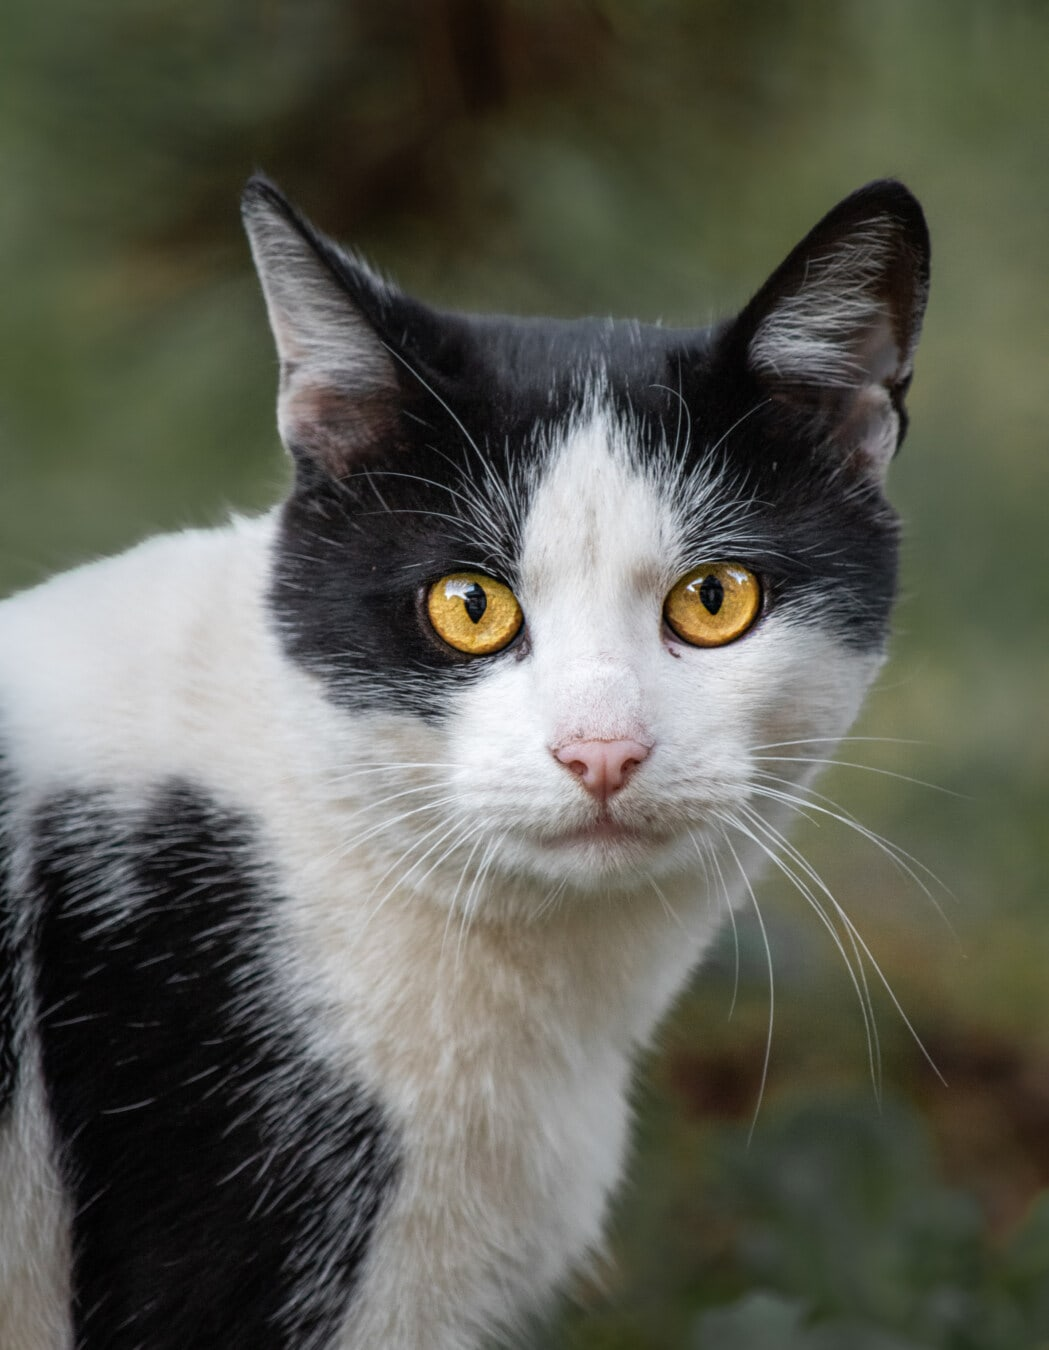
\includegraphics[width=5cm]{image-1080x1350.jpg}
		\caption*{original image}
	\end{minipage}
	\begin{minipage}[t]{0.32\textwidth}
		\centering
		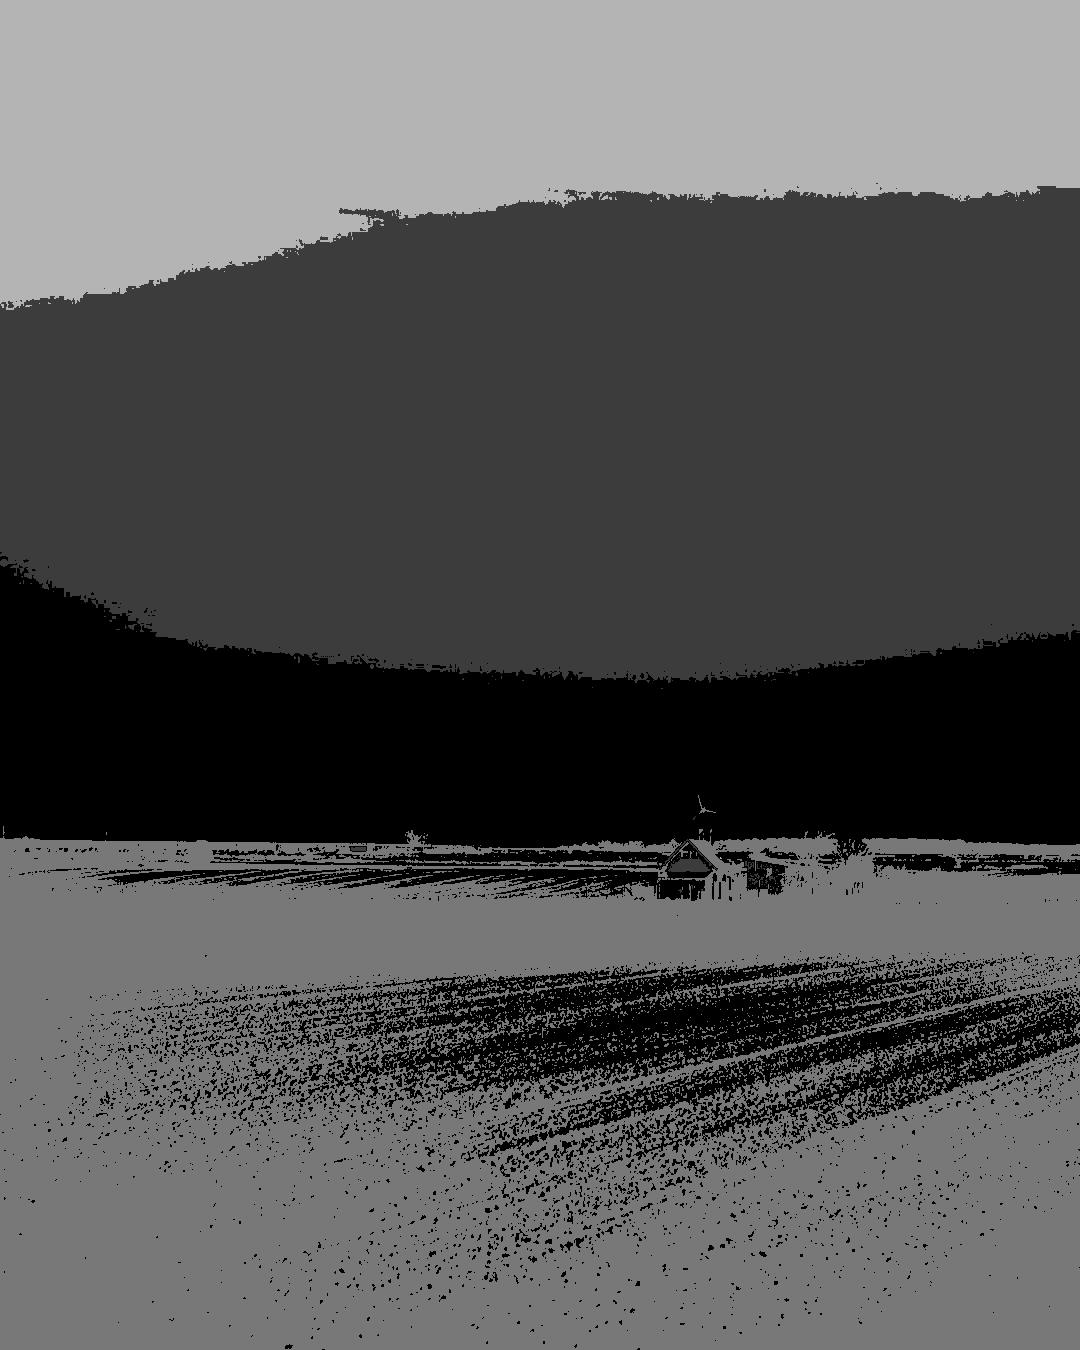
\includegraphics[width=5cm]{cluster4.jpg}
		\caption*{clustering image $k=4$}
	\end{minipage}
	\begin{minipage}[t]{0.32\textwidth}
		\centering
		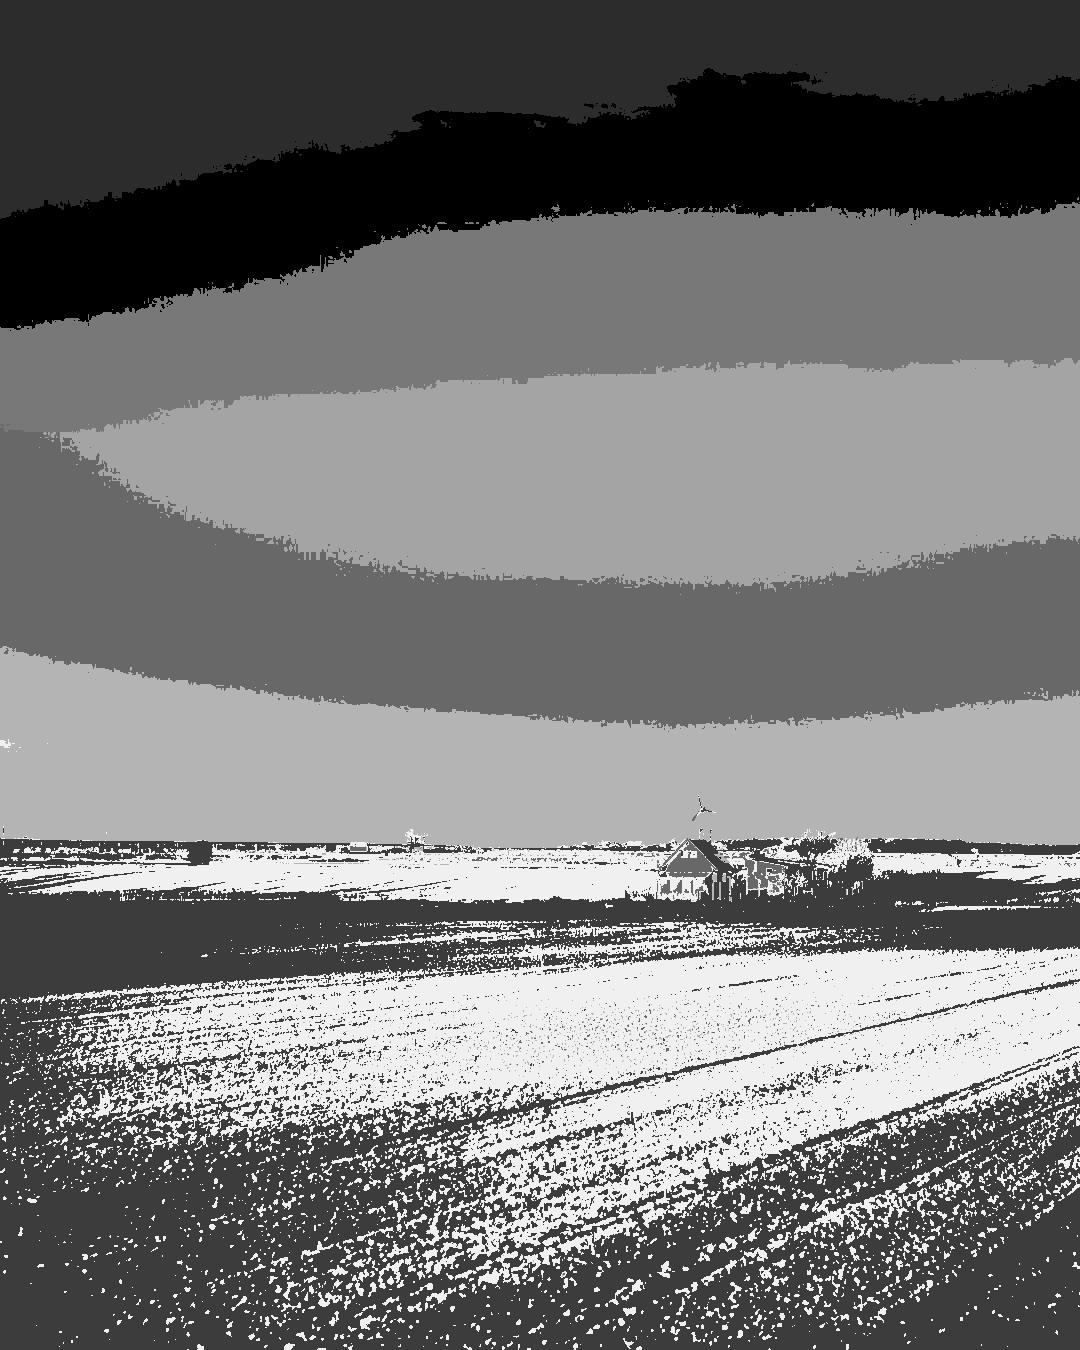
\includegraphics[width=5cm]{cluster8.jpg}
		\caption*{clustering image $k=8$}
	\end{minipage}
	\caption{图像分割结果} \label{fig:figsplit1}
\end{figure}

利用 cv2 库函数分别取 $k=2,4,8,16,64$ 得到的彩色图像分割结果如图 \ref{fig:figsplit2} 所示。

\begin{figure}[htbp]
	\centering
    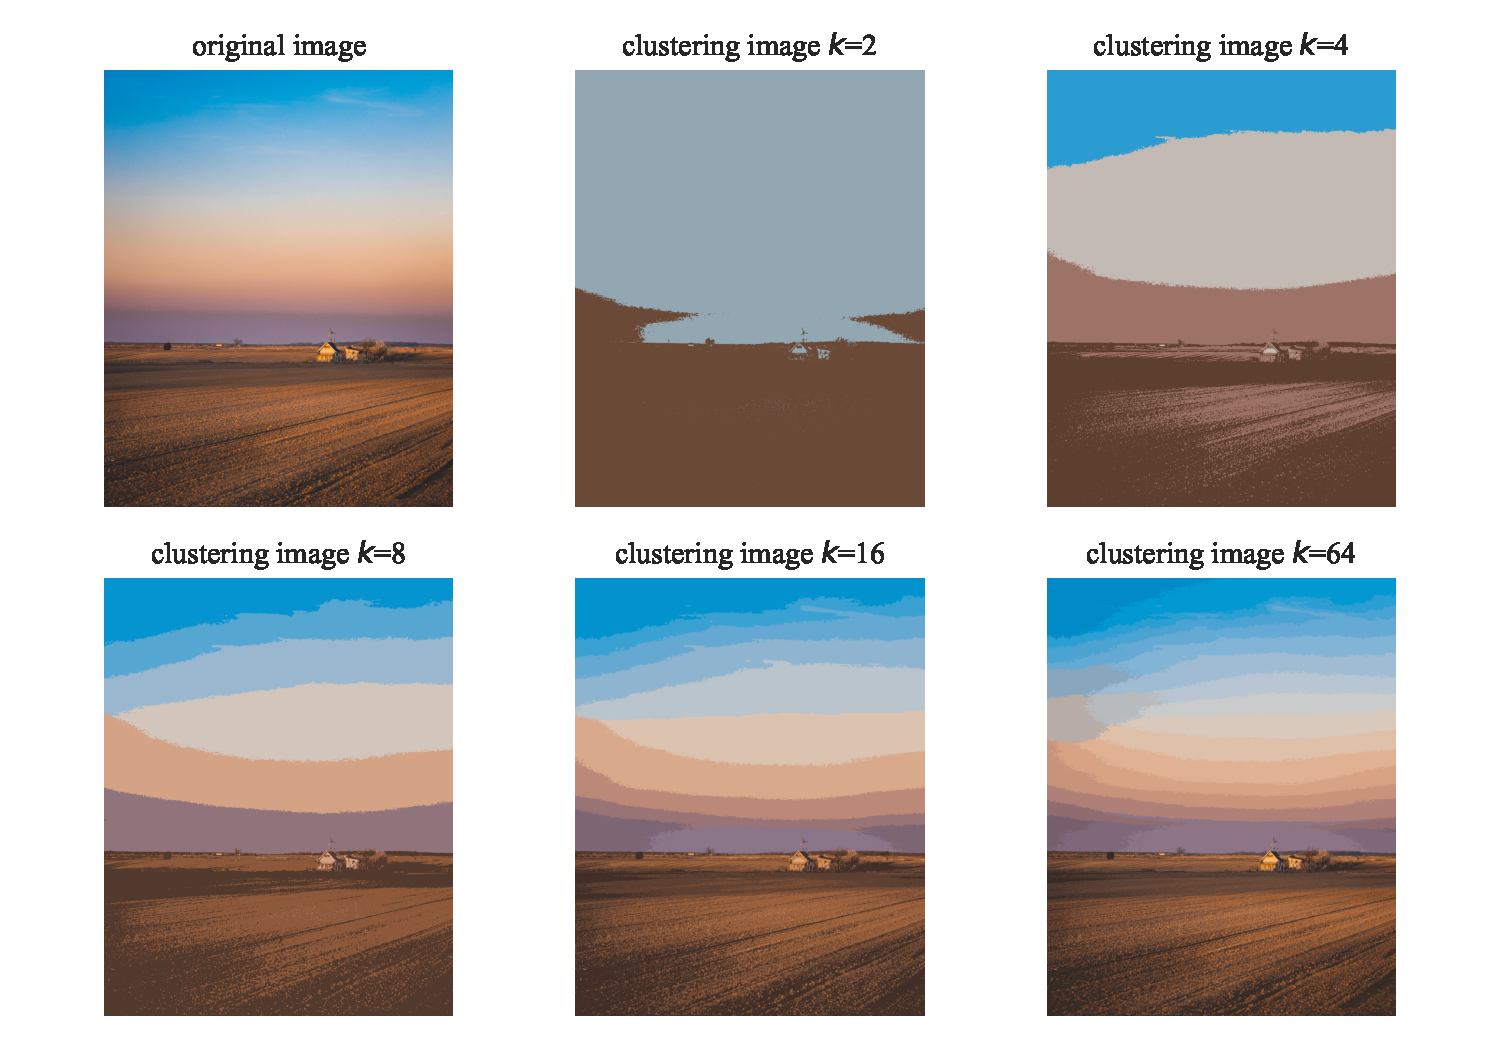
\includegraphics[width=\textwidth]{figsplit.pdf}
    \caption{cv2 彩色图像分割结果} \label{fig:figsplit2}
\end{figure}

可以得出结论,在一定的迭代次数限制下,设置的聚类数越多,图像分割越明显,细节越丰富。并且程序的运行时间会随着聚类数 $k$、最大迭代次数的增加而增加。

\newpage

\includepdfset{pagecommand={\thispagestyle{fancy}}} 
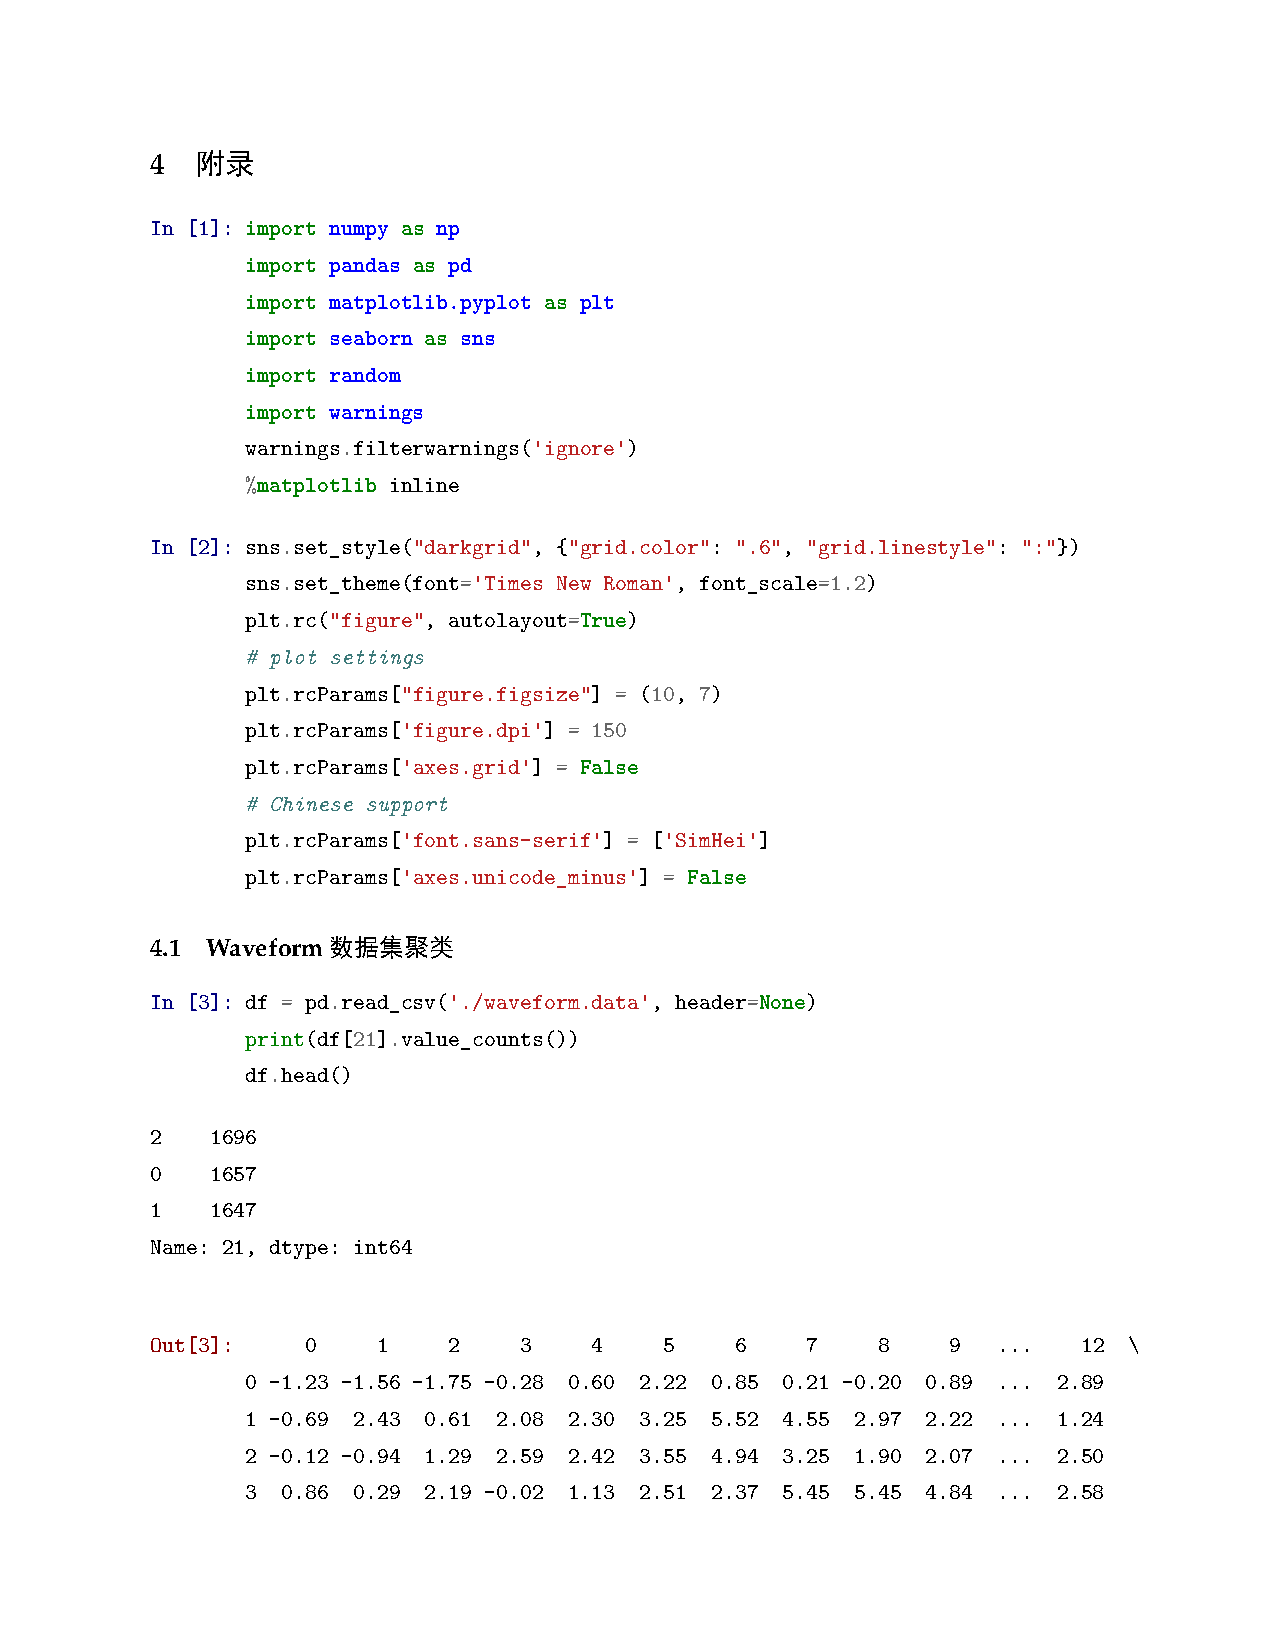
\includepdf[addtotoc={1,section,1,附录,appendix}, pages={1-7}]{Kmeans.pdf}

% % 参考文献,此处以 MLA 引用格式为例

% \begin{thebibliography}{9}
%     \bibitem{1} Clemente, Filipe Manuel, et al. "General network analysis of national soccer teams in FIFA World Cup 2014." \emph{International Journal of Performance Analysis in Sport} 15.1 (2015): 80-96.
%     \bibitem{3} Dijkstra, Edsger Wybe. "A Note on Two Problems in Connexion With Graphs." \emph{Numerische Mathematik} 1(1959):269-271.
%     \bibitem{4} Ahnert, Sebastian E., et al. "Ensemble approach to the analysis of weighted networks.." \emph{Physical Review E} 76.1 (2007).
%     \bibitem{5} Wong, J. A. Hartiganm. A. . "Algorithm AS 136: A K-Means Clustering Algorithm." \emph{Journal of the Royal Statistical Society. Series C (Applied Statistics)} 28.1(1979):100-108.
%     \bibitem{6} Buldu, J. M., et al. "Defining a historic football team: Using Network Science to analyze Guardiola’s F.C. Barcelona." \emph{Scientific Reports} 9.1 (2019): 1-14.
%     \bibitem{7} \emph{Balotelli sends Italy past Germany}. (2012). Retrieved December 10, 2014, from\url{https://www.uefa.com/uefaeuro/season=2012/matches/round=15174/match=2003379/index.html}
%     \bibitem{8} Sigari, Mohamad Hoseyn, et al. "Counterattack detection in broadcast soccer videos using camera motion estimation." \emph{international symposium on artificial intelligence} (2015): 101-106.
%     \bibitem{9} Abdelmahmoud Hassan Elsheikh. \emph{Effect of Leadership Intensity on Integrating Some Formal and Informal Organizational Efforts for Community Development in Khartoum Province}. 2016.
% \end{thebibliography}


% \includepdf[pages={1,2}]{Memo.pdf} 
% 可以直接导入pdf页面
% \newpage
% \begin{appendices}  % 附录环境
% \section{附录}
% \end{appendices}

\end{document}  % 结束